\resizebox{1\textwidth}{!}{%
	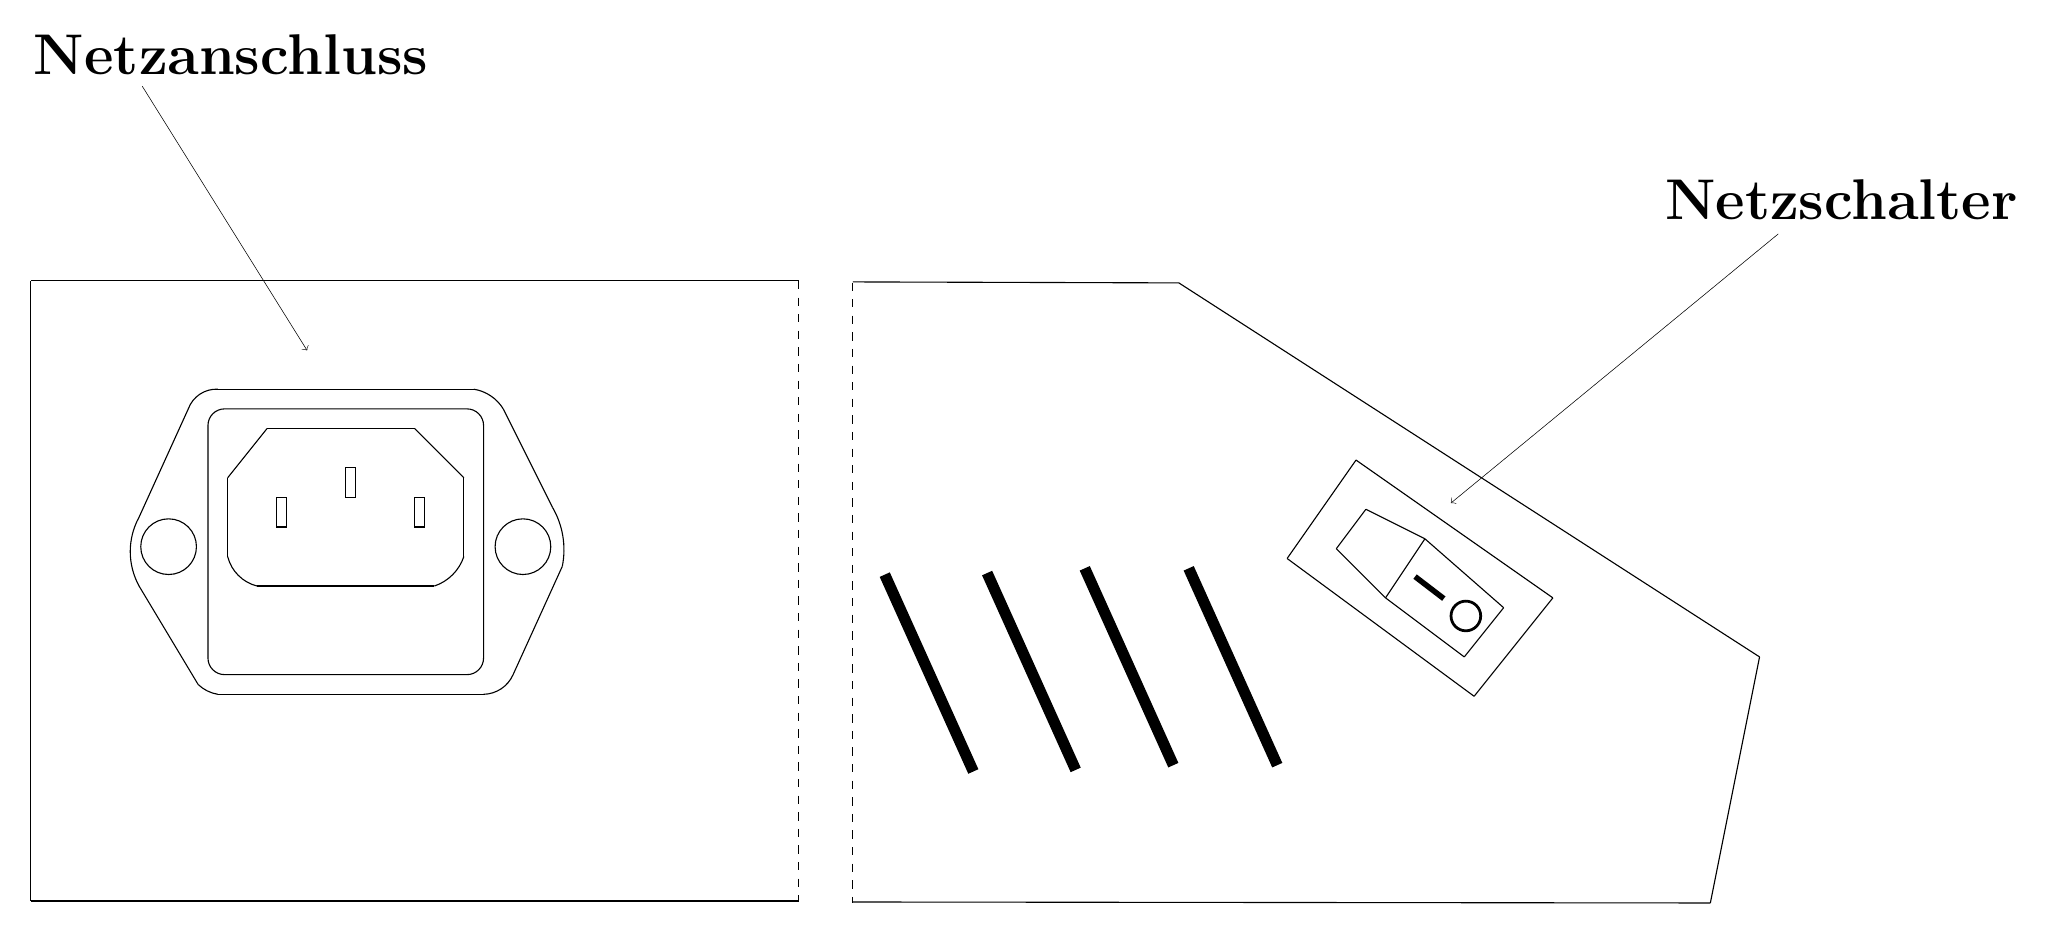
\begin{tikzpicture}
		\tikzstyle{every node}=[font=\fontsize{20pt}{18.5pt}\selectfont]
		\draw [rounded corners=6.0] (-2.875,15.845) rectangle (0.625,12.47);
		\draw (-2.125,15.595) -- (-0.25,15.595);
		\draw (-0.25,15.595) -- (0.375,14.97);
		\draw (0.375,14.97) -- (0.375,13.97);
		\draw (-2.125,15.595) -- (-2.625,14.97);
		\draw (-2.625,14.97) -- (-2.625,13.97);
		\draw (-2.25,13.595) arc[start angle=-103.95, end angle=-166.05, radius=0.5142];
		\draw (0.375,13.97) arc[start angle=-18.54, end angle=-71.46, radius=0.5950];
		\draw (-2.25,13.595) -- (0,13.595);
		\draw (-1.125,15.095) rectangle (-1,14.72);
		\draw (-0.25,14.72) rectangle (-0.125,14.345);
		\draw (-2,14.72) rectangle (-1.875,14.345);
		\draw (-2.75,16.095) -- (0.5,16.095);
		\draw (1.5,14.595) -- (0.875,15.845);
		\draw (1.625,13.845) -- (1,12.47);
		\draw (-3.125,15.845) -- (-3.75,14.47);
		\draw (-3.75,13.595) -- (-3,12.345);
		\draw (-3.125,15.845) arc[start angle=160.00, end angle=87.38, radius=0.3806];
		\draw (0.5,16.095) arc[start angle=81.04, end angle=31.58, radius=0.5387];
		\draw (-2.75,12.22) -- (0.625,12.22);
		\draw (-2.75,12.22) arc[start angle=-99.32, end angle=-133.81, radius=0.4715];
		\draw (1,12.47) arc[start angle=-23.78, end angle=-88.84, radius=0.4190];
		\draw (-3.75,13.595) arc[start angle=-151.28, end angle=-208.72, radius=0.9104];
		\draw (1.5,14.595) arc[start angle=30.29, end angle=-11.37, radius=1.0691];
		\draw (-5.125,17.47) -- (-5.125,9.595);
		\draw (-5.125,17.47) -- (4.625,17.47);
		\draw (-5.125,9.595) -- (4.625,9.595);
		\draw [dashed] (4.625,17.47) -- (4.625,9.595);
		\draw (-3.375,14.095) circle (0.3535533905932738cm);
		\draw (1.125,14.095) circle (0.3535533905932738cm);
		
		\draw (5.314276480000001,17.457513600000002) -- (9.455,17.445);
		\draw (9.455,17.445) -- (16.83,12.695);
		\draw (16.83,12.695) -- (16.205,9.57);
		\draw (16.205,9.57) -- (5.314276480000001,9.582513600000002);
		\draw (11.705,15.195) -- (14.205,13.445);
		\draw (11.705,15.195) -- (10.83,13.945);
		\draw (10.83,13.945) -- (13.205,12.195);
		\draw (14.205,13.445) -- (13.205,12.195);
		\draw (11.83,14.57) -- (12.58,14.195);
		\draw (12.58,14.195) -- (13.58,13.32);
		\draw (13.58,13.32) -- (13.08,12.695);
		\draw (11.83,14.57) -- (11.455,14.07);
		\draw (11.455,14.07) -- (12.08,13.445);
		\draw (12.08,13.445) -- (12.58,14.195);
		\draw (12.08,13.445) -- (13.08,12.695);
		\draw [line width=1pt] (13.1,13.215) circle (0.18838936262746445cm);
		\draw [line width=2pt] (12.455,13.715) -- (12.820127437579773,13.435382312739321);
		
		\draw [line width=4pt] (9.58,13.82) -- (10.705,11.32);
		\draw [line width=4pt] (8.26,13.82) -- (9.385,11.32);
		\draw [line width=4pt] (7.02,13.76) -- (8.145,11.26);
		\draw [line width=4pt] (5.72,13.74) -- (6.845,11.24);
		
		\draw [dashed] (5.305,17.45) -- (5.305,9.575);
		
		\draw [line width=0.2pt, ->] (17.06687071210512,18.06662603651599) -- (12.91034476005441,14.649038031496518);
		\draw [line width=0.2pt, ->] (-3.7097044537799375,19.943181822967784) -- (-1.6160469371914314,16.587171980200914);
		
		\node [fill=white, fill opacity=1, text opacity=1, inner xsep=0.080cm, inner ysep=0.085cm, rounded corners=0.020cm] at (-2.5828756954856815,20.34843241900943) {\textbf{Netzanschluss}};
		\node [fill=white, fill opacity=1, text opacity=1, inner xsep=0.080cm, inner ysep=0.085cm, rounded corners=0.020cm] at (17.86870692899965,18.50556398354723) {\textbf{Netzschalter}};
	\end{tikzpicture}
}%